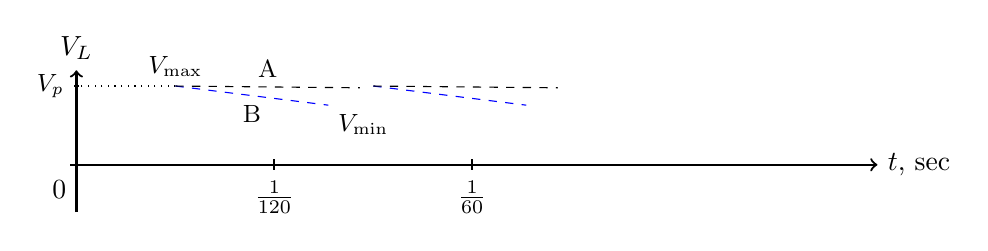
\begin{tikzpicture}[domain=0:8*pi, xscale=.4]
    \draw[->, thick] (-0.2,0) -- (8*pi+.3,0) node[right] {$t$, sec};
    \draw[->, thick] (0,-.6) -- (0,1.2) node[above] {$V_L$};
    \draw[color=red] plot[id=abs-sin,samples=1000] function{abs(sin(.5 * x))};

	% discharge lines
	\draw[color=blue, dashed] (pi,1) -- coordinate (b mid) (8, 0.75680);
	\draw[color=black, dashed] (pi,1) -- coordinate (a mid) (9, 0.97753);
	\node[above] at (a mid) {\small A};
	\node[below] at (b mid) {\small B};
	\draw[color=blue, dashed] (3*pi,1) -- (2*pi+8, 0.75680);
	\draw[color=black, dashed] (3*pi,1) -- (2*pi+9, 0.97753);
	\node[above] at (pi, 1) {\small$V_\mathrm{max}$};
	\node[anchor=north west] at (8, 0.75680) {\small$V_\mathrm{min}$};


	% vertical axis values
	\draw[dotted] (pi, 1) -- (0, 1);
	\draw[thick] (2pt, 1) -- (-2pt, 1) node[anchor=east] {\small$V_p$};

	% tics
	\draw[thick] (0, 2pt) -- (0, -2pt) node[anchor=north east] {0};
	\draw[thick] (2*pi, 2pt) -- (2*pi, -2pt) node[anchor=north] {$\frac{1}{120}$};
	\draw[thick] (4*pi, 2pt) -- (4*pi, -2pt) node[anchor=north] {$\frac{1}{60}$};
\end{tikzpicture}
